\chapter{线虫轮廓的分割、跟踪及特征提取}
	本章将介绍线虫图像处理的流程,包括线虫轮廓的分割、跟踪和特征提取等多个步骤。本章介绍 一种基于背景减除的
	线虫轮廓分割方法,但这种前景提取的方法存在一定的局限性(如:如鲁棒性不足且只能针对静止背景的图像等)。本文将在
	第三章提出一种基于神经网络的前景分割方法,线虫轮廓的解析将在第四章进行介绍。基于轮廓解析的结果,本章提出
	一种基于二分图匹配的跟踪方法。最后,本章将介绍一些在药物筛选和毒理学研究中用于量化线虫行为的特征(如:体长、摆动频率
	和运动速度等)。
\section{线虫图像处理总体方案介绍}
	线虫图像处理的总体流程如图\ref{fig:flow}所示,共分成4个阶段。第一个阶段是从采集到的视频中读取一帧图像,并将
	线虫轮廓覆盖的区域定义为前景,剩下的区域视为背景。这一阶段的输出为一幅二值化的图像,其中1表示前景0表示
	背景。如果是单线虫的跟踪,则第一个阶段的输出则为线虫的轮廓。但考虑到多线虫跟踪过程中多个线虫的轮廓会出现
	相交甚至纠缠在一起,导致因无法区分单个线虫从而跟踪丢失。第二个阶段的任务主要是对多个线虫相交的轮廓进行解析,
	从而得到单个线虫的轮廓。第三个阶段的线虫跟踪是利用线虫轮廓的重心面积等信息找出相邻两帧图像之间线虫轮廓的对应
	关系。第四个阶段主要是利用跟踪到的线虫轮廓计算出线虫体长、运动速度等信息。

		\begin{figure}[h]
	  \centering
	  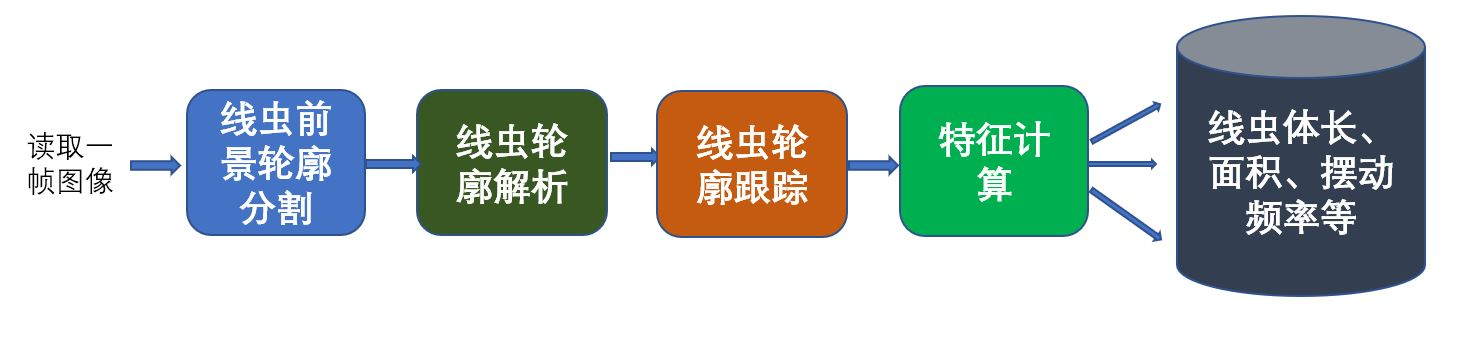
\includegraphics[width=14cm]{figure/chap3/flow.jpg}
	  % \hspace{1cm}
	  % 
\includegraphics[width=4cm]{example/sjtulogo.jpg}
	  \bicaption[这里将出现在插图索引中]
		{线虫图像处理总体流程图}
		{The flow chart of C.elegans image processing}
	  \label{fig:flow}
	\end{figure}
\section{基于背景减除方法的线虫轮廓分割}
	通过背景减除方法实现前景轮廓提取需要对背景进行建模,假设在一幅图像中每个像素的取值具有空间独立性
	,只与最近的T个历史像素取值相关。在时间$t$历史像素可以表示为$h_T=\{x^{(t)},\dots,x^{(t-T)}\}$,
	则每个像素的取值用一个包含M个高斯的混合高斯概率函数来建模,公式\ref{eq:gmm}中$FG$表示像素属于前景,$BG$表示
	该像素属于背景。$\hat{u}_1,\dots,\hat{u}_M$和$\hat{\sigma}_1^2,\dots,\hat{\sigma}_M^2$分别表示混合高斯模型中的待估参数均值和方差。
	$\hat{\pi}_m$表示高斯权重且所有权重相加等于1。
	\begin{equation}
		p(\vec{x}|h_T,BG+FG)= \sum_{m=1}^{M} \hat{\pi}_{m}N(\vec{x};\hat{u}_m,\hat{\sigma}_m^2I)\label{eq:gmm}
	\end{equation}
	当在时刻t得到一个新像素值$\vec{x}^{(t)}$时,模型参数将如下方式更新,其中$\vec{\delta}_m=\vec{x}^{(t)}-\hat{u}_m$,
	$a=1/T$。并将与新像素值$\vec{x}^{(t)}$最近的高斯分量对应的$o_m^{(t)}$设置为1其他设置为0。
	\begin{equation}
		\hat{\pi}_m \leftarrow \hat{\pi}_m +a(o_m^{(t)}-\hat{\pi}_m) \label{eq:updata}
	\end{equation}
	\begin{equation}
		\hat{u}_m \leftarrow \hat{u}_m +o_m^{(t)}(a/\hat{\pi}_m)\vec{\delta}_m \label{eq:updata1}
	\end{equation}
	\begin{equation}
		\hat{\sigma}_m^2 \leftarrow \hat{\sigma}_m^2 +o_m^{(t)}(a/\hat{\pi}_m)(\vec{\delta}_m^T\vec{\delta}_m-\hat{\sigma}_m^2) \label{eq:updata2}
	\end{equation}
	将M个高斯分量按照权重从大到小排序,则背景模型可以通过前B个最大的高斯分量来近似。
	\begin{equation}
		p(\vec{x}|h_T,BG) \sim \sum_{m=1}^{B} \hat{\pi}_{m}N(\vec{x};\hat{u}_m,\hat{\sigma}_m^2I)\label{eq:bg}
	\end{equation}
	如图\ref{fig:bgsub}所示基于混合高斯
	模型的背景减除方法与简单的帧间差分法相比,背景减除的方法能够显著的减少前景轮廓提取的不连续分割的性能
	更好。用一个$5\times5$的核对提取到的前景轮廓进行形态学闭运算得到的结果如图\ref{fig:bgsub:close}所示。
	最后,运用OTSU二值化算法就可以得到最终的线虫前景轮廓如图\ref{fig:bgsub:bin}所示。

	
% \begin{figure*}
% \centering
% \subfigure[Input]{
% \begin{minipage}[b]{0.23\linewidth}
% 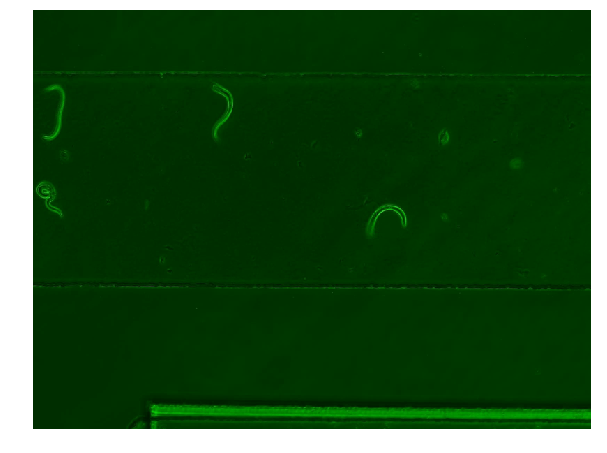
\includegraphics[width=1\linewidth]{figure/chap3/worm.png}\vspace{4pt}
% 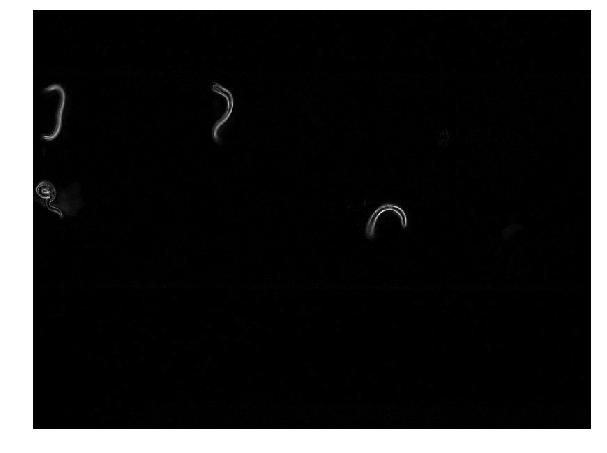
\includegraphics[width=1\linewidth]{figure/chap3/bgsub.png}\vspace{4pt}
% 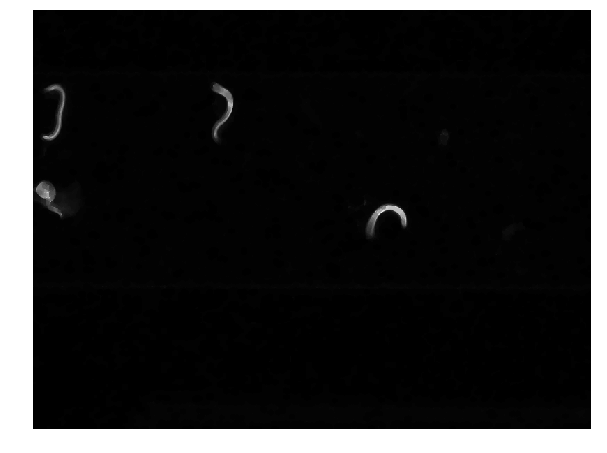
\includegraphics[width=1\linewidth]{figure/chap3/close.png}
% \end{minipage}}
% \subfigure[CE]{
% \begin{minipage}[b]{0.23\linewidth}
% 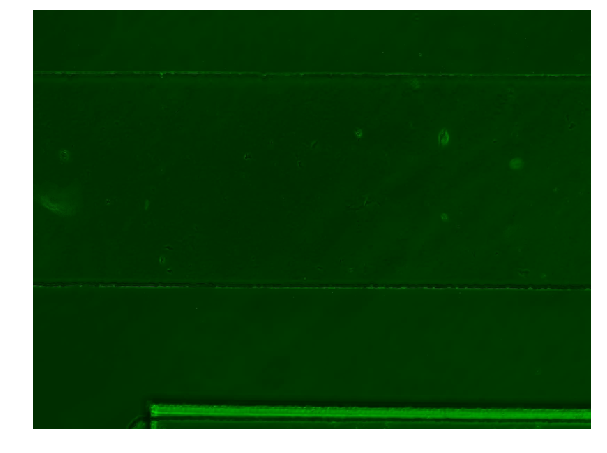
\includegraphics[width=1\linewidth]{figure/chap3/bg.png}\vspace{4pt}
% 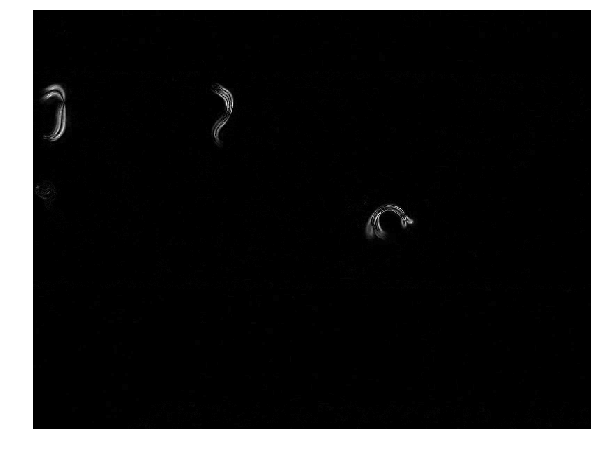
\includegraphics[width=1\linewidth]{figure/chap3/difffra.png}\vspace{4pt}
% 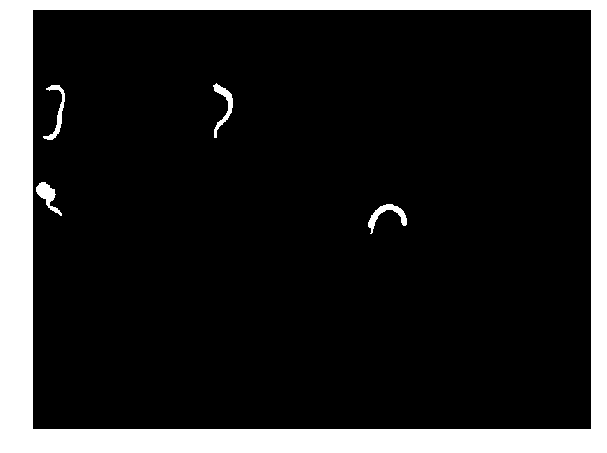
\includegraphics[width=1\linewidth]{figure/chap3/otsu.png}
% \end{minipage}}
% \caption{description of figure}
% \end{figure*}
\begin{figure}[h]
  \centering
  \begin{subfigure}{0.4\textwidth}
    \centering
    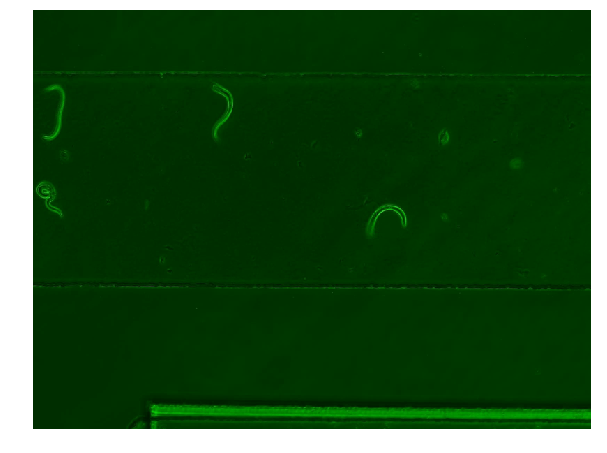
\includegraphics[width=1\linewidth]{figure/chap3/worm.png}
    \caption{待处理线虫图像}
	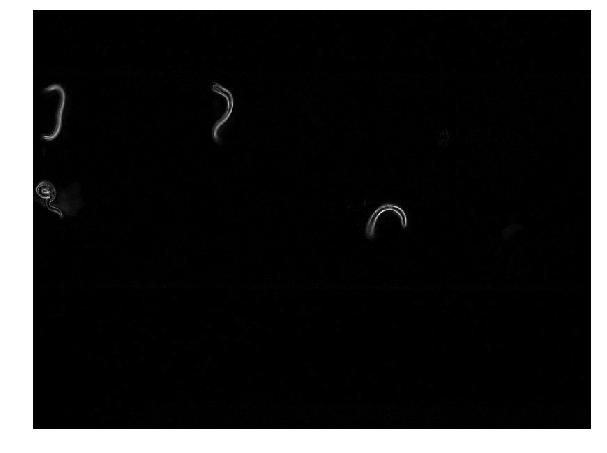
\includegraphics[width=1\linewidth]{figure/chap3/bgsub.png}
	\caption{基于混合高斯模型背景减除图片}
	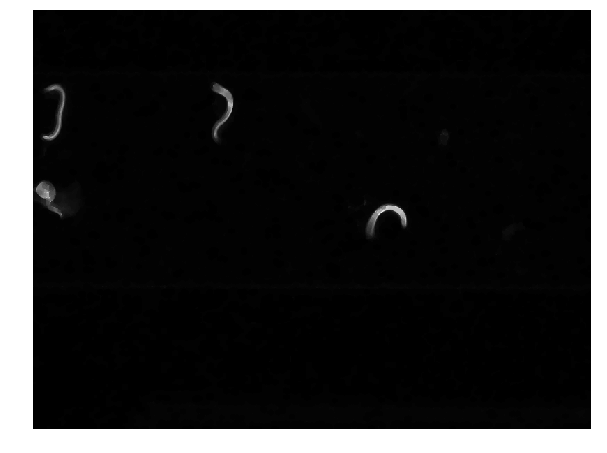
\includegraphics[width=1\linewidth]{figure/chap3/close.png}
	\caption{对背景减除得到的图像闭运算}\label{fig:bgsub:close}
  \end{subfigure}
  \hspace{4em}
  \begin{subfigure}{0.4\textwidth}
    \centering
    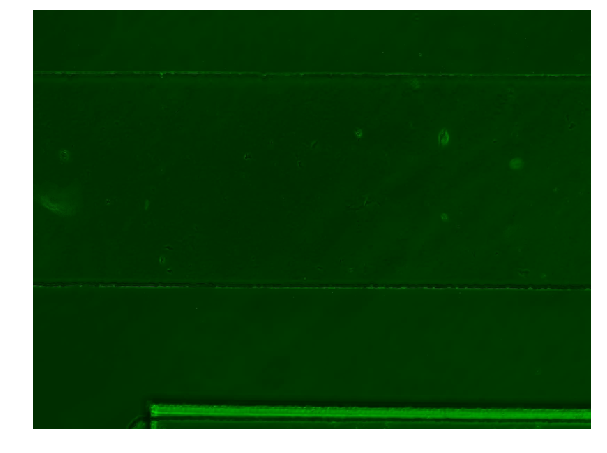
\includegraphics[width=1\linewidth]{figure/chap3/bg.png}
    \caption{基于混合高斯模型建模的背景图}
	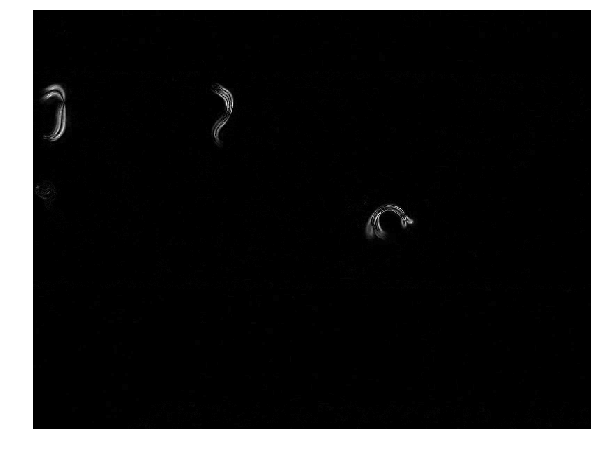
\includegraphics[width=1\linewidth]{figure/chap3/difffra.png}
	\caption{帧间差分法结果图}
	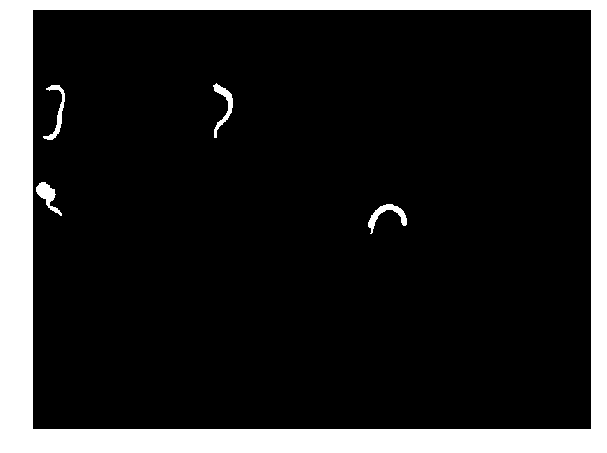
\includegraphics[width=1\linewidth]{figure/chap3/otsu.png}
	\caption{OTSU阈值处理后的二值图}\label{fig:bgsub:bin}
  \end{subfigure}
  \bicaption{前景提取过程中的图片}{The images in the foreground object extraction}
  \label{fig:bgsub}
\end{figure}
\section{线虫轮廓的跟踪}
	由于线虫通体透明,跟踪起来比较困难,本文采用了一种简单有效的跟踪策略。首先经过
	线虫前景轮廓提取和线虫轮廓解析等步骤后,可以得到每一帧图像里所有线虫的轮廓。由
	公式\ref{eq:m}和公式\ref{eq:xy}可以计算出轮廓的重心坐标。
	\begin{equation}
		m_{ji}=\sum_{x,y}I_{x,y}x^iy^j \label{eq:m}
	\end{equation}
	\begin{equation}
		\vec{x}=\frac{m_{10}}{m_{00}},\quad \vec{y}=\frac{m_{01}}{m_{00}}\label{eq:xy}
	\end{equation}
	假设当前帧有n个轮廓,上一帧
	图像有m个轮廓,由每个轮廓的重心坐标可以得到一个$n\times m$的距离矩阵用公式\ref{eq:matrix}
	表示。
		\begin{equation}
                        D=\left[
                \begin{matrix}
                 d_{11}      & d_{12}      & \cdots & d_{1m}      \\
                 d_{21}      & d_{22}      & \cdots & d_{2m}      \\
                 \vdots & \vdots & \ddots & \vdots \\
                 d_{n1}      & d_{n2}      & \cdots & d_{nm}      \\
                \end{matrix}
                \right]\label{eq:matrix}
    \end{equation}
	矩阵中$d_{ij}$表示当前帧中的第i个轮廓的重心到上一帧中第j个轮廓的重心之间的距离。通过
	公式\ref{eq:min}可以得到相邻两帧图像中线虫轮廓之间的对应关系。即如果相邻两帧图像中两个
	轮廓重心之间的距离最短,则可以认为是同一个线虫。
		\begin{equation}
        index(i)=\mathop{\arg\min}_{j} d_{ij}\label{eq:min}
		\end{equation}
	但事实上由于轮廓分割的不完美以及图像噪声的影响
	,这一策略往往会失效。因此,通过最近邻搜索的方式来实现线虫的跟踪要满足以下的约束条件,当这两个
	条件之一不满足时,则认为跟踪丢失,此时应该分配一个新的trackID给当前的轮廓。算法\ref{algo:worm_track}
	是描述了线虫跟踪算法的实现思路。
	
	\begin{itemize}
	  \item 相邻两帧图像中同一只线虫的轮廓面积的相对变化应该小于一个阈值。
	  \item 根据线虫运动的最大速度,同一只线虫在相邻两帧图像中轮廓的重心之间的距离应该小于一个阈值。
	\end{itemize}

\begin{algorithm}
\caption{跟踪初始化程序}
\label{algo:initial_track}
\begin{algorithmic}[1]
	\Require $Worm\_data$双重列表,$Worm\_data[i][j]$表示第$i$帧图像中第$j$只线虫。
	\Ensure 输出$trackID$
	\Function {Initiate\_tracking}{$Worm\_data$}
		\State $FirstFrame\_WormData \gets Worm\_data[0]$
		\For{$i = 0 \to FirstFrame\_WormData.length-1$}
			\State $cur\_worm \gets FirstFrame\_WormData[i]$
			\State $cur\_worm.trackID \gets GetNewTrackID()$
		\EndFor
\EndFunction
\end{algorithmic}
\end{algorithm}

\begin{algorithm}[H]
\caption{线虫跟踪程序}
\label{algo:worm_track}
\begin{algorithmic}[1]
	\Require $Worm\_data$双重列表,$Worm\_data[i][j]$表示第$i$帧图像中第$j$只线虫。
	\Ensure 输出$trackID$
	\Function {Worm\_tracking}{$Worm\_data$}
		\State $Initiate\_tracking(Worm\_data)$
		\For{$frame_index = 1 \to Worm\_Data.length-1$}
			\State $PreFrame\_WormData \gets Worm\_Data[frame_index-1] $
			\For{$worm\_index =0 \to Worm\_Data[frame_index].length-1$}
\algstore{WormTracking}
\end{algorithmic}
\end{algorithm}
\begin{algorithm}[H]
\begin{algorithmic}[1]
\algrestore{WormTracking}
		
				\State $cur\_worm \gets Worm\_Data[frame\_index][worm\_index]$
				\State $dist\_array \gets Compute\_distance(cur\_worm,PreFrame\_WormData)$
				\State $min\_index \gets Get\_min\_index(dist\_array)$
				\State $Nearest\_worm \gets PreFrame\_WormData[min\_index]$
				\If{$\small{\frac{|Nearest\_worm.Area-cur\_worm.Area|}{Nearest\_worm.Area}<\delta \quad \text{and}  \quad dist\_array[min\_index]< \sigma}$}
					\State $cur\_worm.trackID \gets Nearest\_worm.trackID$
				\Else
					\State $cur\_worm.trackID \gets GetNewTrackID( )$
				\EndIf
			\EndFor
		\EndFor
\EndFunction
\end{algorithmic}
\end{algorithm}
\section{线虫的特征提取}
\subsection{线虫轮廓中间脊线提取}


\section{本章小结}


